\documentclass{IEEEtran}

\usepackage[utf8]{inputenc}
\usepackage{graphicx}
\usepackage{amsmath}
\usepackage{siunitx}
\usepackage{listings}
\usepackage[citestyle=ieee,sorting=none,bibencoding=utf8,backend=biber]{biblatex}

\usepackage{algorithm}
\usepackage[noend]{algpseudocode}

\graphicspath{{images/}}
\bibliography{bibliography}
\makeatletter
\def\BState{\State\hskip-\ALG@thistlm}
\makeatother

\author{J.R. Powers-Luhn}
\title{Ridge}
\date{October 16th, 2018}

\begin{document}
\maketitle

\begin{abstract}

\end{abstract}

\section{Introduction}

\section{Methodology}

\section{Results}

\begin{centering}
\begin{figure}
\centering
\begin{center}
	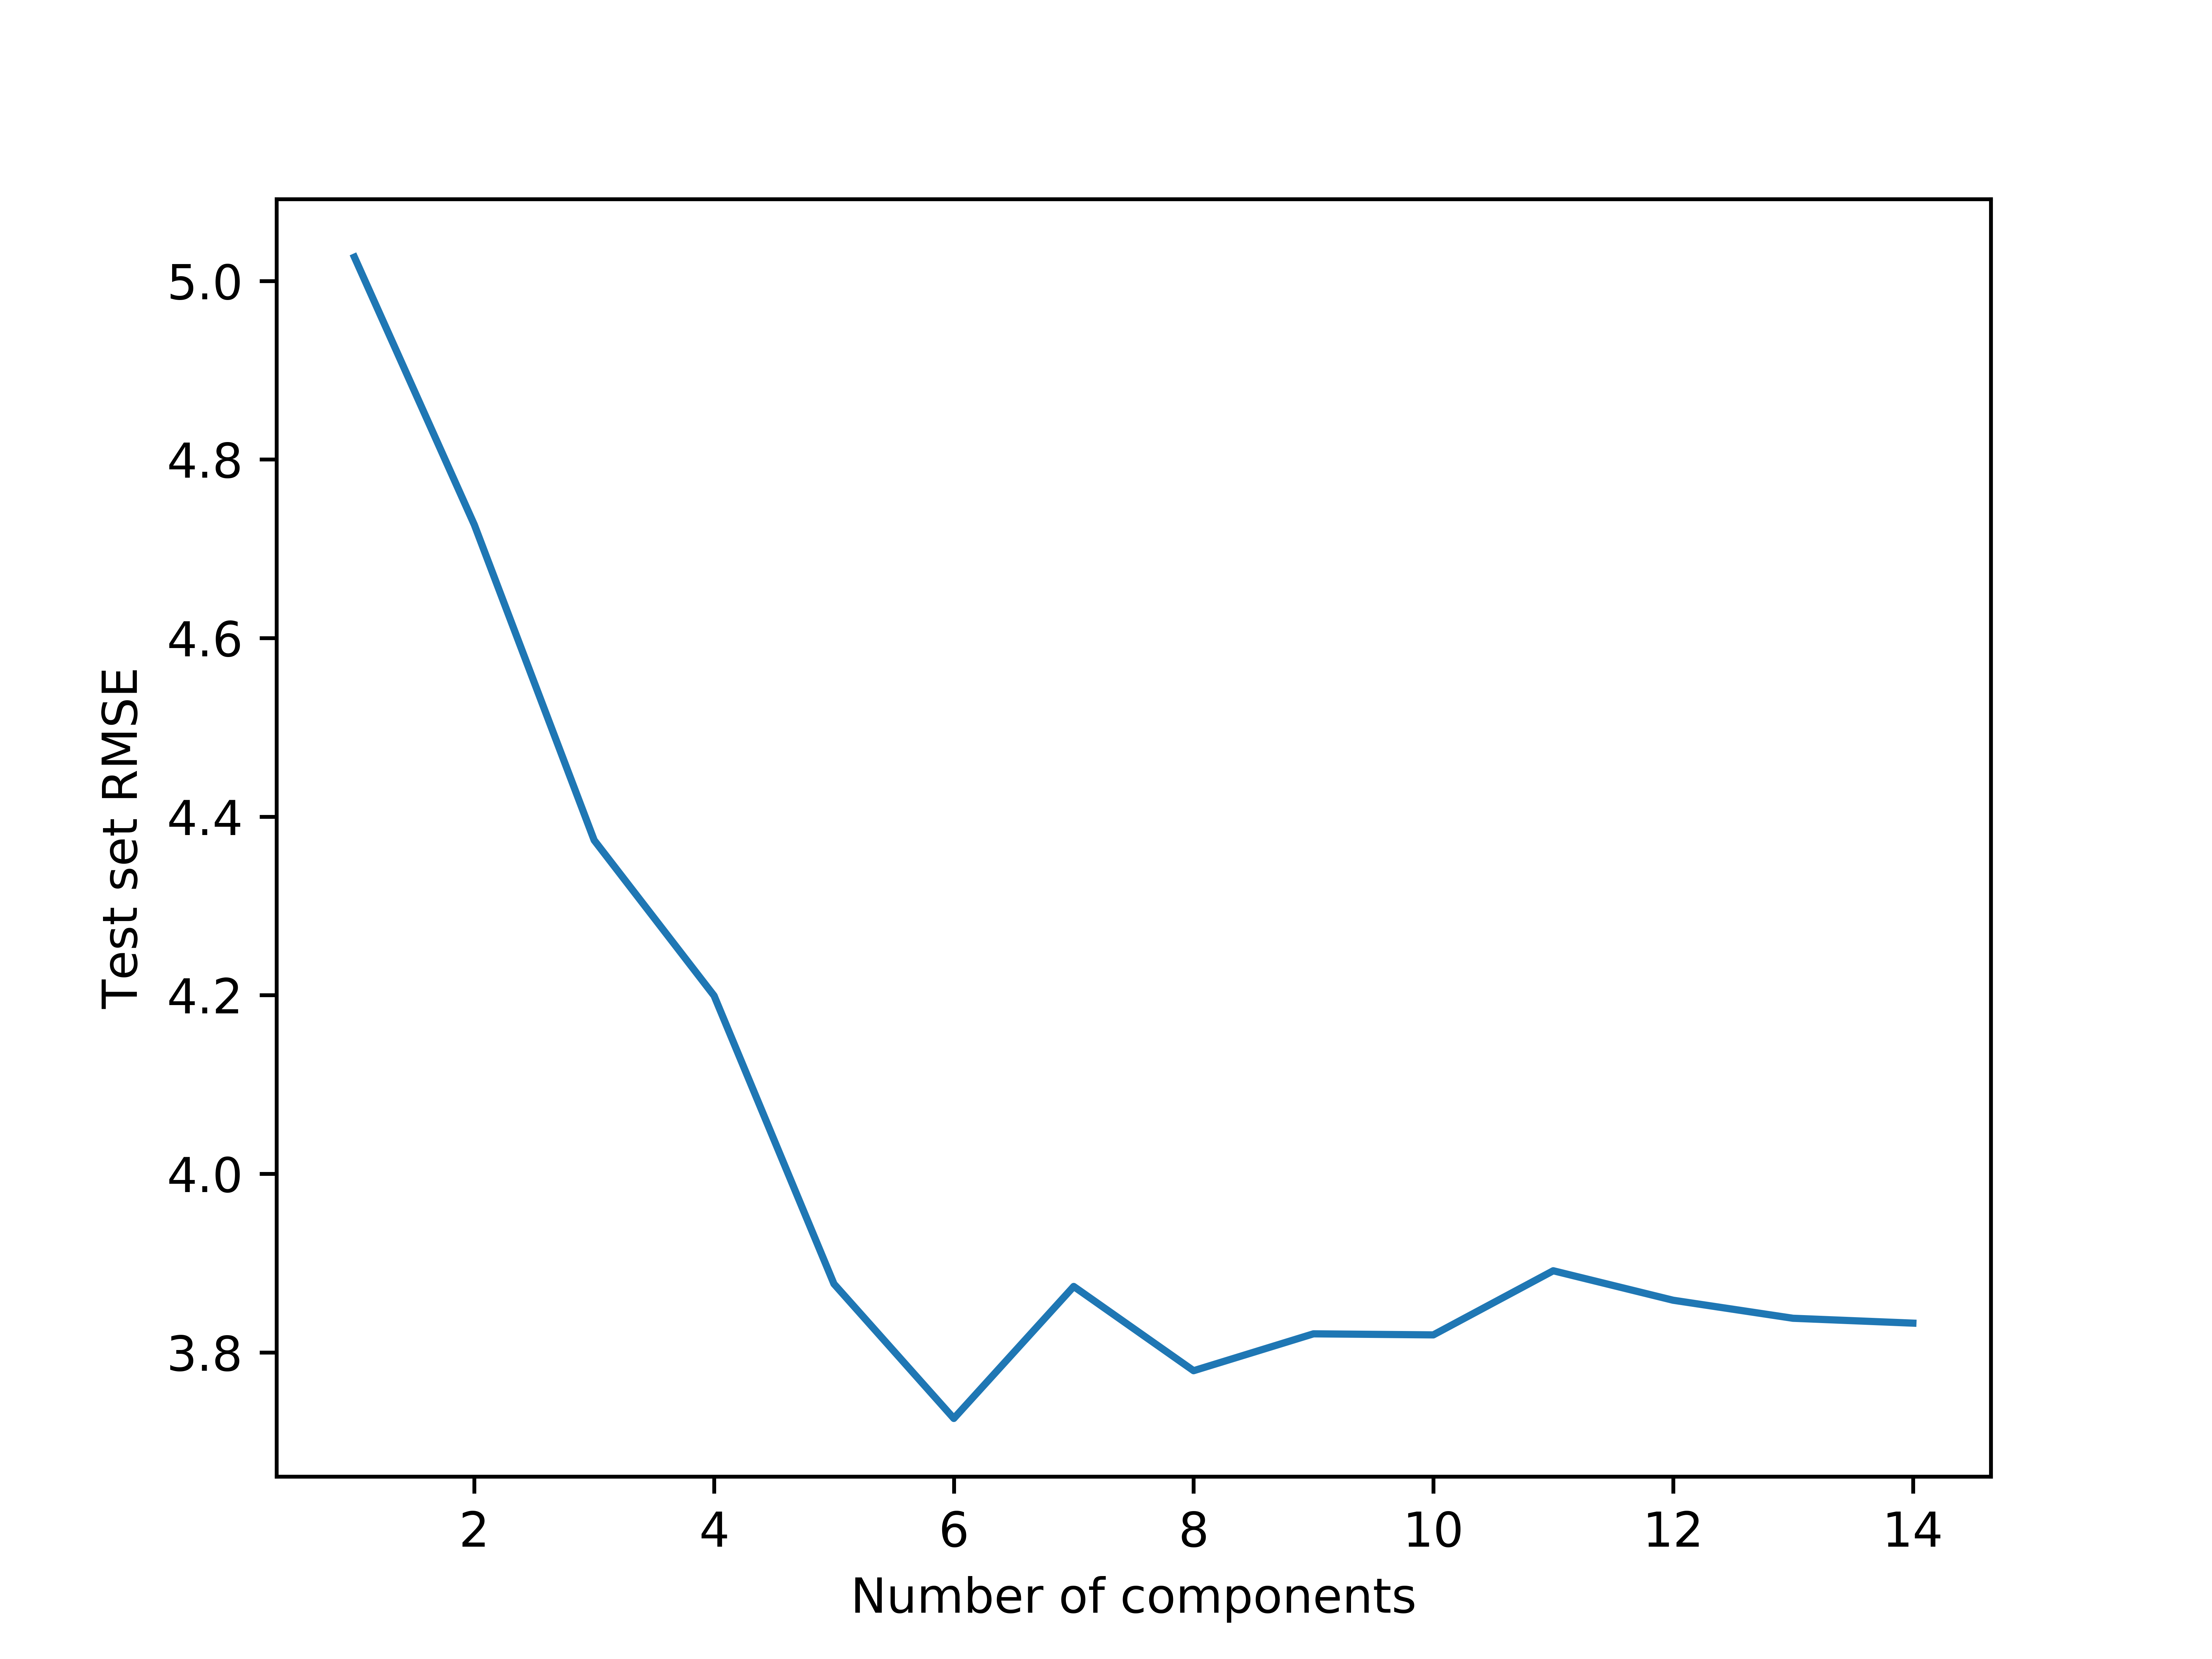
\includegraphics[width=0.48\textwidth]{rmse_vs_number_components}
	\caption{Performance of the partial least squares regression as a function of the number of latent variables. Training error always goes down since each additional component necessarily fits the residual data not explained by earlier components. Testing error reaches and then oscillates around a minimum value.\label{fig:rmse_vs_number_components}}
\end{center}
\end{figure}
\end{centering}

\section{Conclusions}

Partial least squares was used to generate a model that could predict body fat percentage with a root mean squared error of \num{4.35}. This outperformed models previously generated using linear regression and principal component regression even without the generation of polynomial, inverse, or interaction terms. PLS latent variables were compared to PCR principal components and determined to be fundamentally different in spite of the visual similarity. The smaller number of components required to minimize test set error was shown to be a natural result of selecting latent variables in order of maximum input/output covariance. This provides real-world advantages by simplifying model input and increasing the stability of models.

\printbibliography

\onecolumn
\section{Appendix}
Python code used to perform calculations and generate graphics.
\lstset{frame=single}
\lstinputlisting[language=python]{hw06.py}

\end{document}